% SSU Data Dash 2026 submission draft. Replace the link placeholders before submission.
\documentclass[10pt]{article}
\usepackage[margin=1.8cm]{geometry}
\usepackage{graphicx,booktabs,hyperref}
\graphicspath{{../figures/}}
\setlength{\parskip}{3pt}
\setlength{\parindent}{0pt}
\title{SSU Data Dash 2026: Toronto Fourcast}
\author{Yan Cui, Jiayi Guan, Shengde Wang, Ziang Chen}
\date{}

\begin{document}
\maketitle
\vspace{-1.2em}

\textbf{Five-minute video:} \url{[Add unlisted YouTube URL]}\hfill
\textbf{Code and predictions:} \url{[Add GitHub repository URL]}

\section*{Summary}
We trained separate gradient-boosted models for the off-market and list-aware questions. In six monthly walk-forward validations from December 2025 through May 2026, the models reached MdAPE of 10.60\% off-market and 4.36\% list-aware across 10,069 homes per track. These are below the starter benchmarks of 20.8\% and 7.3\%, respectively. Community, municipality, and house-style categories helped the model distinguish homes with similar sizes and coordinates; the remaining errors are largest for high-priced off-market homes.

\section{Data and features}
We used the provided 150,000 synthetic sales from January 2021 through May 2026. Numeric features include the midpoint of the listed square-footage range, bedrooms, washrooms, parking, latitude, longitude, and months since January 2021. We added the provided property type, house style, municipality, and community as categorical features. The off-market feature set never uses list price; the list-aware feature set adds it. Garage and lot dimensions were tested, but paired validation did not show a reliable improvement, so we excluded them. We used no outside data. Listing remarks and third-party AVM estimates are absent from the prediction files, so they were not used.

\section{Models}
Both tracks use scikit-learn's histogram gradient-boosting regressor trained on log sale price. The model handles the categorical columns directly. Each validation model learns its category vocabulary from that fold's training sales; unseen categories at prediction time become missing values. The list-aware model receives list price because that field exists at prediction time. The off-market model does not.

\section{Validation and results}
We used the starter's expanding, month-by-month protocol. For each month from December 2025 to May 2026, the model trained only on sales before that month and predicted that month's sales. We did not use hidden test prices. The intervals below come from a bootstrap over validation homes; they do not account for homes sharing market conditions within a month.

\begin{table}[h]
\centering\small
% Written by `python run.py report`. Do not edit by hand: rerun the command instead.
\begin{tabular}{lrccc}
\hline
Track & Homes & MdAPE \% (95\% CI) & MAPE \% (95\% CI) & Median signed error \% \\
\hline
off-market & 10,069 & 10.45 (10.22--10.70) & 13.05 (12.81--13.29) & -0.07 \\
list-aware & 10,069 & 4.34 (4.24--4.42) & 5.51 (5.42--5.60) & +0.61 \\
\hline
\end{tabular}

\caption{Walk-forward validation. MdAPE is median absolute percentage error; MAPE is mean absolute percentage error. Parentheses show 95\% home-level bootstrap intervals.}
\end{table}

Against the starter baselines, off-market MdAPE fell from 20.8\% to 10.60\% and list-aware MdAPE from 7.3\% to 4.36\%. The reductions were consistent in all six months. A paired bootstrap against our feature-only model estimated a further MdAPE reduction of 3.80 percentage points off-market (95\% interval: 3.52 to 4.12) and 0.19 points list-aware (0.14 to 0.24) after adding the three categorical features.

\section{Where errors remain}
\begin{figure}[h]
\centering
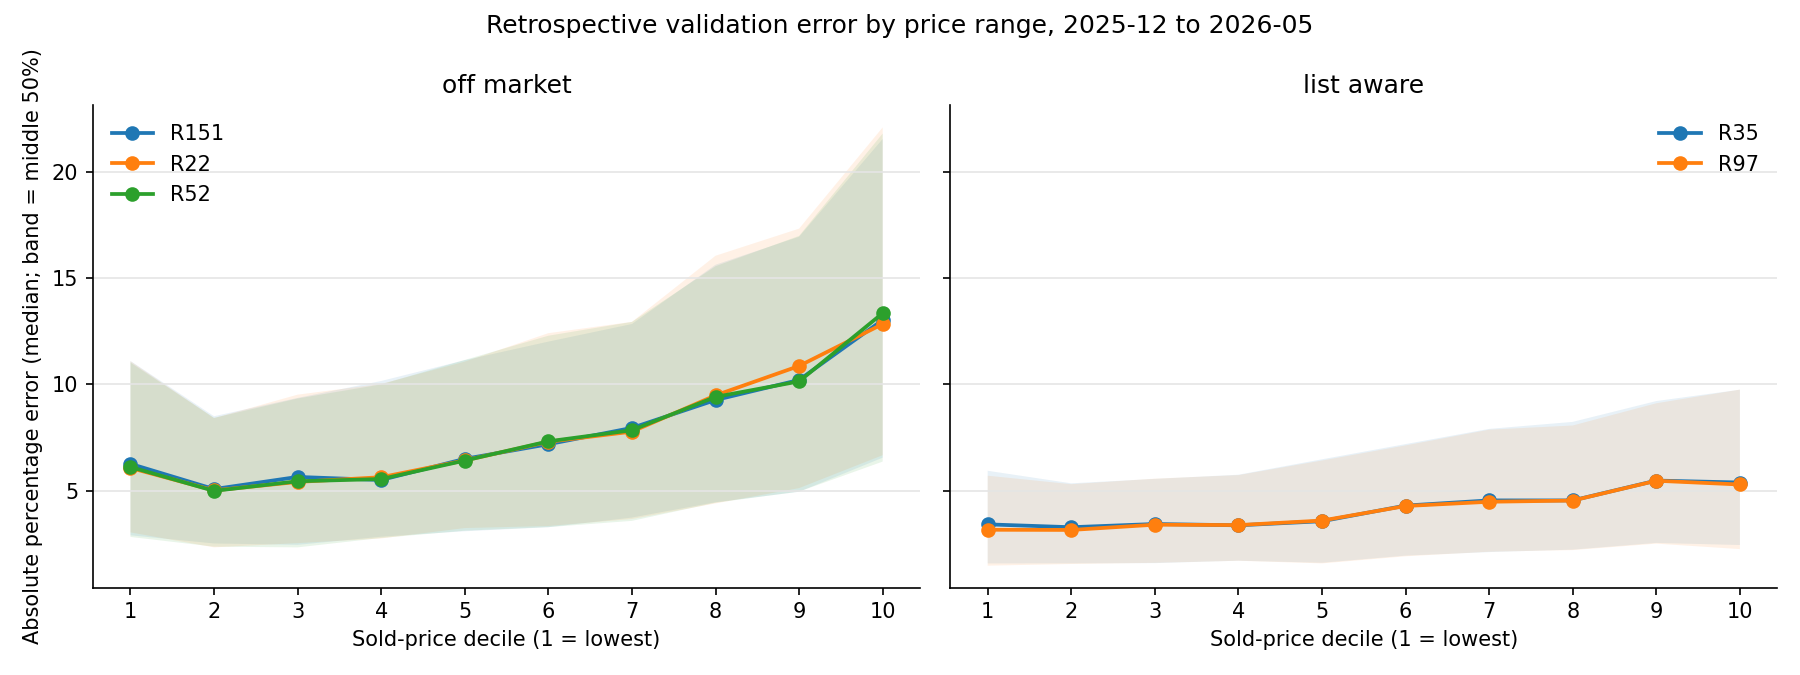
\includegraphics[width=0.82\linewidth]{error_by_price_range.png}
\caption{Absolute percentage error by shared sold-price decile; line is the median and band is the middle 50\%.}
\end{figure}
\vspace{-0.6em}
Off-market error is highest for the cheapest and most expensive deciles (MdAPE 13.10\% and 16.55\%), compared with roughly 8\% to 12\% across the middle. List-aware error also rises in the top decile (5.79\%, versus 3.67\% in the second and third deciles). By property type, off-market Co-op Apt has 14.33\% MdAPE, but this group has only 48 validation homes. These segment results describe the synthetic validation set and do not establish why individual errors occur.

\section{Limitations}
The validation covers six months and may not match the hidden June--September 2026 distribution. Home-level bootstrap intervals understate uncertainty if errors are correlated within months. The competition data are synthetic: its communities and coordinates do not map to real Toronto locations, and these results should not be presented as a live-market valuation service. We would next test time-aware community comparables and segment calibration using the same forward-only validation.

\section*{Outside data}
None.

\section*{Reproducing the predictions}
From a clean clone, install the pinned requirements and run:
\begin{verbatim}
python -m pip install -r requirements.txt
python run.py validate
python run.py report
python run.py predict
python run.py check
\end{verbatim}

\end{document}
